\documentclass{beamer}
\setbeamersize{text margin left=3mm,text margin right=3mm}


\usepackage[backend=bibtex, natbib=true, style=authoryear]{biblatex}% \usepackage[style=authoryear]{natbib}
% \bibliographystyle{plain}
\addbibresource{bibliography}

\usepackage{amsmath, bm, amssymb, bbm}
\usepackage{tcolorbox}

\usepackage{subcaption}
\usepackage{graphicx}
\graphicspath{{./../code}}
\usepackage{xcolor}
\usepackage{hyperref}
\hypersetup{
    colorlinks=true,
    linkcolor=blue,
    filecolor=magenta,
    urlcolor=cyan,
    pdftitle={Overleaf Example},
    pdfpagemode=FullScreen,
    }
\usepackage{multirow}

\usepackage{tikz}
\usetikzlibrary{matrix,positioning,arrows.meta,arrows,fit,backgrounds,decorations.pathreplacing}

\tikzset{
  mymat/.style={ matrix of math nodes, text height=2.5ex, text
    depth=0.75ex, text width=6.00ex, align=center, column
    sep=-\pgflinewidth, nodes={minimum height=5.0ex}
  },
  mymats/.style={ mymat, nodes={draw,fill=#1}
  },
  mymat2/.style={
    matrix of math nodes, text height=1.0ex, text depth=0.0ex, minimum
    width=5ex, % text
    width=7.00ex, align=center, column sep=-\pgflinewidth
  },
}

\usetikzlibrary{shapes.geometric, arrows, backgrounds, scopes}
\usepackage{pgfplots} \pgfplotsset{width=6.75cm, compat=newest}
\usepackage[utf8]{inputenc} \DeclareUnicodeCharacter{2212}{−}
\usepgfplotslibrary{groupplots,dateplot}
\usetikzlibrary{patterns,shapes.arrows}



\usepackage{tikzsymbols}
\usetheme{Boadilla}
\usecolortheme{seahorse}
\newcommand{\thetab}{\boldsymbol{\theta}}
\newcommand{\xb}{\boldsymbol{x}}
\DeclareMathOperator*{\argmin}{arg\,min}
\DeclareMathOperator*{\argmax}{arg\,max}



\newcommand{\when}[1]{\mathbbm{1}_{#1}}




\title[RAM: Regionally Additive Models]{Regionally Additive Models: Explainable-by-design models minimizing feature interactions}
\subtitle{}
\author[Gkolemis, Vasilis] % (optional)
{Vasilis Gkolemis\inst{1,2} \and Anargiros Tzerefos\inst{1} \and Theodore Dalamagas\inst{1} \and Eirini Ntoutsi\inst{3} \and Christos Diou\inst{2}}

\institute[]{
  \inst{1} ATHENA Research and Innovation Center
  \and %
  \inst{2} Harokopio University of Athens
  \and
  \inst{3} Universitat der Bundeswehr Munchen
}

\date{September 2023, Turin, Italy}


% ------------------------------------------------------------
\begin{document}
\frame{\titlepage}
%---------------------------------------------------------

\begin{frame}
  \frametitle{Generalized Additive Models (GAMs)}

  Wikipedia says:
  \begin{quote}
    In statistics, a generalized additive model (GAM) is a generalized linear model in which the \textcolor<2-4>{red}{response} variable depends \textcolor<3-4>{blue}{linearly} on unknown \textcolor<4>{cyan}{smooth functions of some predictor variables}.
  \end{quote}
  \noindent\makebox[\linewidth]{\rule{\paperwidth}{0.4pt}}
  \[
    \only<2>{\textcolor{red}{y}}
    \only<3>{\textcolor{red}{y} = \textcolor{blue}{\cdot + \ldots + \cdot}}
    \only<4>{\textcolor{red}{y} = \textcolor{cyan}{f_1(x_1)} \textcolor{blue}{+ \ldots +} \textcolor{cyan}{f_D(x_D)}}
  \]
\end{frame}


\begin{frame}
  \frametitle{Introductory Example}

  Output/target variable:

  \begin{itemize}
  \item \(y_{\mathtt{bike-rentals}}\): the expected number of bike rentals per hour
  \end{itemize}

  \noindent\makebox[\linewidth]{\rule{\paperwidth}{0.4pt}}

  Input/covariates:

  \begin{itemize}
  \item \(x_{\mathtt{temperature}}\): temperature per hour
  \item \(x_{\mathtt{humidity}}\): humidity per hour
  \item \(x_{\mathtt{is\_weekday}}\): if it is weekday or weekend
  \end{itemize}

  \noindent\makebox[\linewidth]{\rule{\paperwidth}{0.4pt}}

  Let's fit a GAM:

  \[y = f_1(x_{\mathtt{temperature}}) + f_2(x_{\mathtt{humidity}}) + f_3(x_{\mathtt{is\_weekday}}) \]

\end{frame}

\begin{frame}
  \frametitle{GAMs - Interpretability (1)}

  $f_1(x_{\mathtt{temperature}})$

  \noindent\makebox[\linewidth]{\rule{\paperwidth}{0.4pt}}

  \begin{figure}[ht]
    \centering
    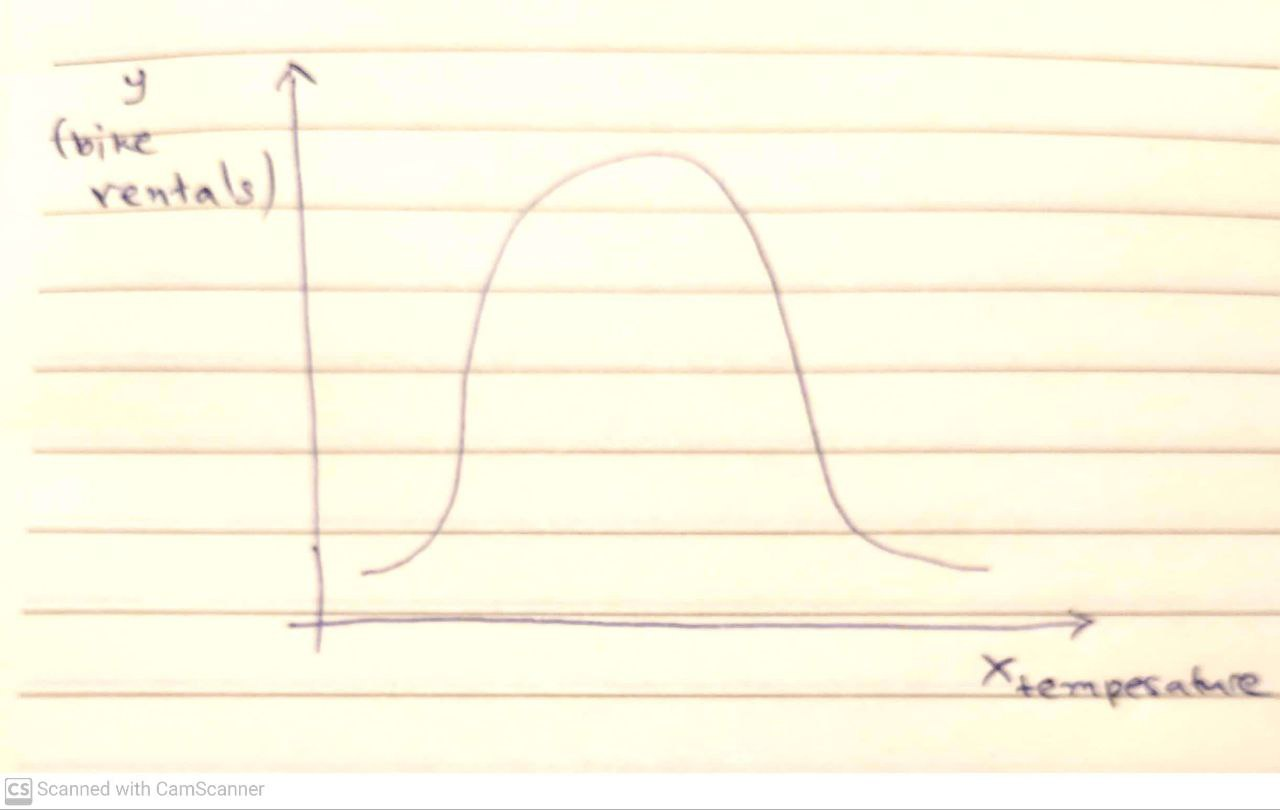
\includegraphics[width=0.7\textwidth]{./figures/gam_temperature.jpg}
  \end{figure}

\end{frame}


\begin{frame}
  \frametitle{GAMs - Interpretability (2)}

  $f(x_{\mathtt{humidity}})$

  \noindent\makebox[\linewidth]{\rule{\paperwidth}{0.4pt}}

  \begin{figure}[ht]
    \centering
    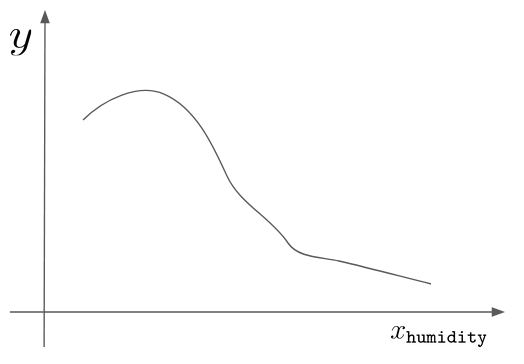
\includegraphics[width=0.7\textwidth]{./figures/gam_humidity.jpg}
  \end{figure}

\end{frame}

\begin{frame}
  \frametitle{GAMs - Interpretability (3)}

  $f(x_{\mathtt{is\_weekday}})$

  \noindent\makebox[\linewidth]{\rule{\paperwidth}{0.4pt}}

  \begin{figure}[ht]
    \centering
    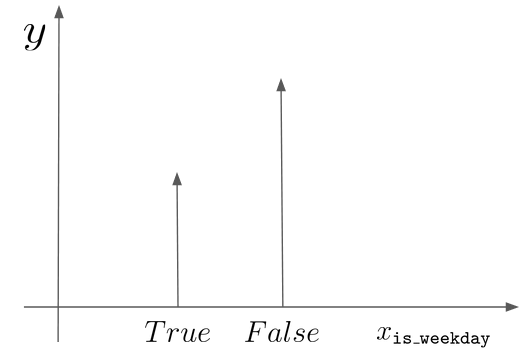
\includegraphics[width=0.7\textwidth]{./figures/gam_is_weekday.jpg}
  \end{figure}

\end{frame}

\begin{frame}
  \frametitle{GAMs - Interpretability (4)}

  GAMs is explainable!

  \noindent\makebox[\linewidth]{\rule{\paperwidth}{0.4pt}}

  \begin{figure}[ht]
    \centering
    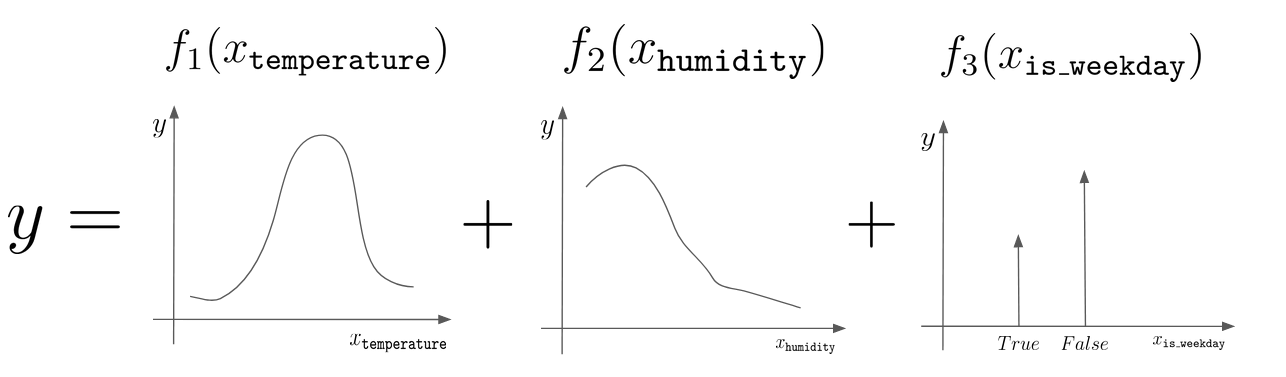
\includegraphics[width=1\textwidth]{./figures/gam.png}
  \end{figure}

\end{frame}


\begin{frame}
  \frametitle{GAMs - Limitations/Extensions}

  Limitations:
  \begin{itemize}
  \item<2-> temperature has different effect on week-days vs weekends
  \item<3-> Cause: go to work vs go sightseeing
  \item<4-> Solution 1: Add pairwise term \(f(x_{\mathtt{temperature}}, x_{\mathtt{is\_weekday}})\) \only<8> {\textcolor{green}{Explainable}}
  \item<5-> Solution 2: Model two conditional terms
    \begin{itemize}
    \item<5-> \(f(x_{\mathtt{temperature}} | weekday )\) \only<8> {\textcolor{green}{Explainable}}
    \item<5-> \(f(x_{\mathtt{temperature}} | weekend )\) \only<8> {\textcolor{green}{Explainable}}
    \end{itemize}
  \end{itemize}

  \noindent\makebox[\linewidth]{\rule{\paperwidth}{0.4pt}}
  Extensions:
  \begin{itemize}
  \item<6-> \textcolor<8>{green}{Solution 1: \(GA^2M = \) GAM + pairwise interactions (\href{https://www.cs.cornell.edu/~yinlou/papers/lou-kdd13.pdf}{Yin Lou et. al})}
  \item<7-> \textcolor<8>{green}{Solution 2: \(RAM = \) GAM at subregions}
  \end{itemize}

\end{frame}


\begin{frame}
  \frametitle{$RA^{(2)}Ms$ go even beyond}

  $GA^2M$s Limitations:
  \begin{itemize}
  \item<2-> Have you ever ridden a bike in a cold day with humidity?
  \item<3-> If it is weekend, let's see a movie instead!
  \item<4-> But if it workday? and bike is the only transport?
  \item<5-> model $f(x_{\mathtt{temperature}}, x_{\mathtt{humidity}}, x_{\mathtt{is\_weekday}})$? \only<6-9> {\textcolor{red}{Not explainable}}
  \end{itemize}

  \noindent\makebox[\linewidth]{\rule{\paperwidth}{0.4pt}}

  $RA^{(2)}Ms$ solve that:

  \begin{itemize}
  \item<7-> \(f(x_{\mathtt{temperature}}, x_{\mathtt{humidity}} | x_{\mathtt{is\_weekday}}) \rightarrow RA^2M\) \only<9> {\textcolor{green}{Explainable}}
    \item<8-> \(f(x_{\mathtt{temperature}}| x_{\mathtt{humidity}} = \{high, low\}, x_{\mathtt{is\_weekday}}) \rightarrow\) RAM with two conditions \only<9> {\textcolor{green}{Explainable}}
  \end{itemize}

\end{frame}


\begin{frame}
  \frametitle{RAM on toy example}

  \[f(\xb) = 8x_2\when{x_1 > 0}\when{x_3=0}\]

  \[ x_1, x_2 \sim \mathcal{U}(-1,1), x_3 \sim Bernoulli(0,1)\]

  \noindent\makebox[\linewidth]{\rule{\paperwidth}{0.4pt}}

  \begin{figure}[htbp]
    \centering
    \begin{subfigure}{0.32\textwidth}
        \centering
        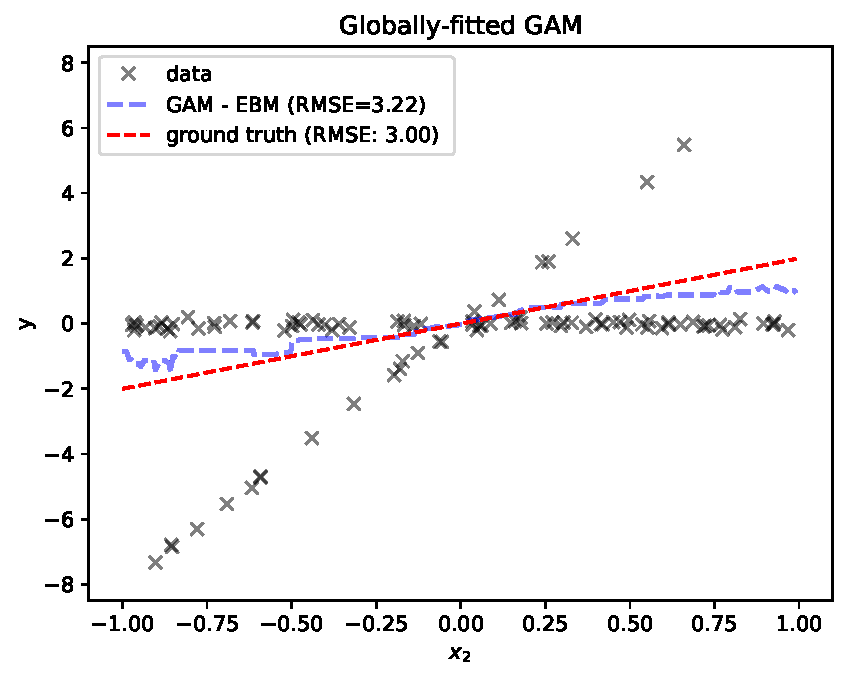
\includegraphics[width=\textwidth]{figures/global_GAM}
        \caption{\(f_2(x_2)\)}
        \label{subfig:global_gam}
    \end{subfigure}
    \begin{subfigure}{0.32\textwidth}
        \centering
        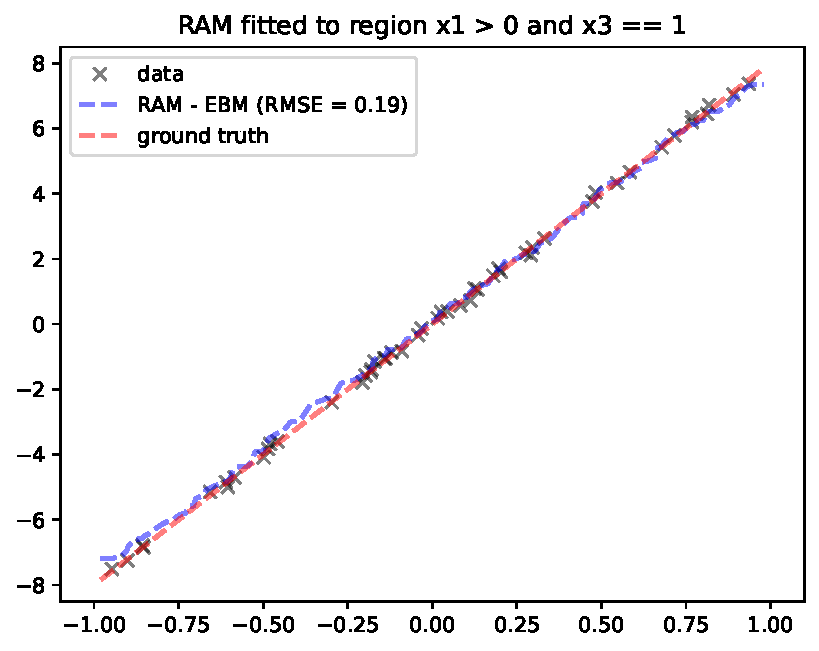
\includegraphics[width=\textwidth]{figures/regional_gam_subreg_1}
        \caption{\(f_2(x_2) \when{x_1 > 0 \text{ and } x_3 = 1}\)}
        \label{subfig:regional_gam_1}
    \end{subfigure}
    \begin{subfigure}{0.32\textwidth}
        \centering
        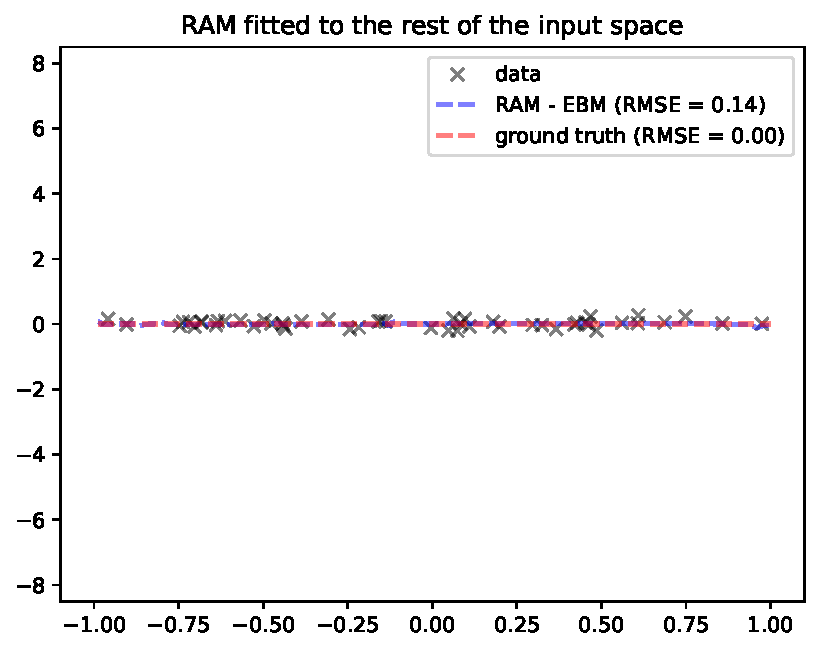
\includegraphics[width=\textwidth]{figures/regional_gam_subreg_2}
        \caption{\(f_2(x_2) \when{x_1 \leq 0 \text{ or } x_3 \neq 1}\)}
        \label{subfig:regional_gam_2}
    \end{subfigure}
    \caption{(Left) GAM, (Middle and Right) RAM}
    \label{fig:ram_example}
\end{figure}
\end{frame}


\begin{frame}
  \frametitle{How RAM works}

  3-step approach:

  \begin{itemize}
    \item<2-4> Fit a black-box model to learn complex feature interactions
      \begin{itemize}
      \item it should be differentiable
      \item neural network is a good option
      \end{itemize}
    \item<3-4> Use a Regional Effect method to isolate the important interactions
      \begin{itemize}
      \item \href{https://givasile.github.io/assets/pdf/gkolemis23_rhale.pdf}{RHALE - Gkolemis et. al}
      \item \href{https://arxiv.org/pdf/2306.00541.pdf}{Feature Interactions - Herbinger et. al}
      \item finds which features $f(x_i)$ should be split into subregions $f(x_i | x_j \lessgtr \tau)$
      \end{itemize}
    \item<4> Fit a univariate function on each detected subregion
      \begin{itemize}
      \item learn all $f(x_i | x_j \lessgtr \tau)$
      \end{itemize}
  \end{itemize}
\end{frame}

\begin{frame}
  \frametitle{Step 1}
  \begin{itemize}
  \item Fit a black-box model to capture all complex structures
    \begin{itemize}
    \item it should be differentiable
    \item A neural network is a good option
  \end{itemize}
\end{itemize}
\end{frame}

\begin{frame}
  \frametitle{Step 2}
  \begin{itemize}
  \item Regional Effect method to find important interactions
    \begin{itemize}
    \item \href{https://givasile.github.io/assets/pdf/gkolemis23_rhale.pdf}{RHALE - Gkolemis et. al}
    \item \href{https://arxiv.org/pdf/2306.00541.pdf}{Feature Interactions - Herbinger et. al}
    \end{itemize}
  \item Idea:
    \begin{itemize}
    \item Feature effect is the average effect of each feature $x_s$ on the output $y$
    \item It is computed by averaging the instance-level effects
    \item Heterogeneity $\mathcal{H}$ (or uncertainty) measures the deviation of the instance-level effects from the average effect
    \item we want to split the dataset in subgroups in order to minimize the heterogeneity
    \end{itemize}
  \item In mathematical terms:
    \[\underbrace{\mathcal{H}(f_i(x_i))}_{\mathcal{H}\text{ before split}} >> \underbrace{\mathcal{H}(f_i(x_i | x_j > \tau)) + \mathcal{H}(f_i(x_i | x_j \leq \tau))}_{\text{sum of } \mathcal{H} \text{ after split}}\]
  \end{itemize}
\end{frame}

\begin{frame}
  \frametitle{Step 3}
  \begin{itemize}
  \item Step 2 defines a new feature space \(\mathcal{X}^{\mathtt{RAM}}\)
  \item Every feature is split to $T_s$ subregions which are defined by $\mathcal{R}_{st}$:
  \end{itemize}

\begin{equation}
\label{eq:ram_feature_space}
\begin{aligned}
\mathcal{X}^{\mathtt{RAM}} &= \{x_{st} | s \in \{1, \ldots, D\}, t \in \{1, \ldots, T_s\}\} \\
x_{st} &= \begin{cases}
x_s, & \text{if } \mathbf{x_{/s}} \in \mathcal{R}_{st} \\
0, & \text{otherwise}
\end{cases}
\end{aligned}
\end{equation}

\begin{itemize}
\item Fit a univariate function on each subregion:
\end{itemize}

\begin{equation}
\label{eq:ram_formulation2}
f^{\mathtt{RAM}}(\mathbf{x})= c + \sum_{s,t} f_{st}(x_{st}) \quad \mathbf{x} \in \mathcal{X}^{\mathtt{RAM}}
\end{equation}

\end{frame}

\begin{frame}
  \frametitle{Bike Sharing dataset}
  Predict bike-rentals per hour
  \noindent\makebox[\linewidth]{\rule{\paperwidth}{0.4pt}}
\begin{figure}[htbp]
    \centering
    \begin{subfigure}{0.32\textwidth}
        \centering
        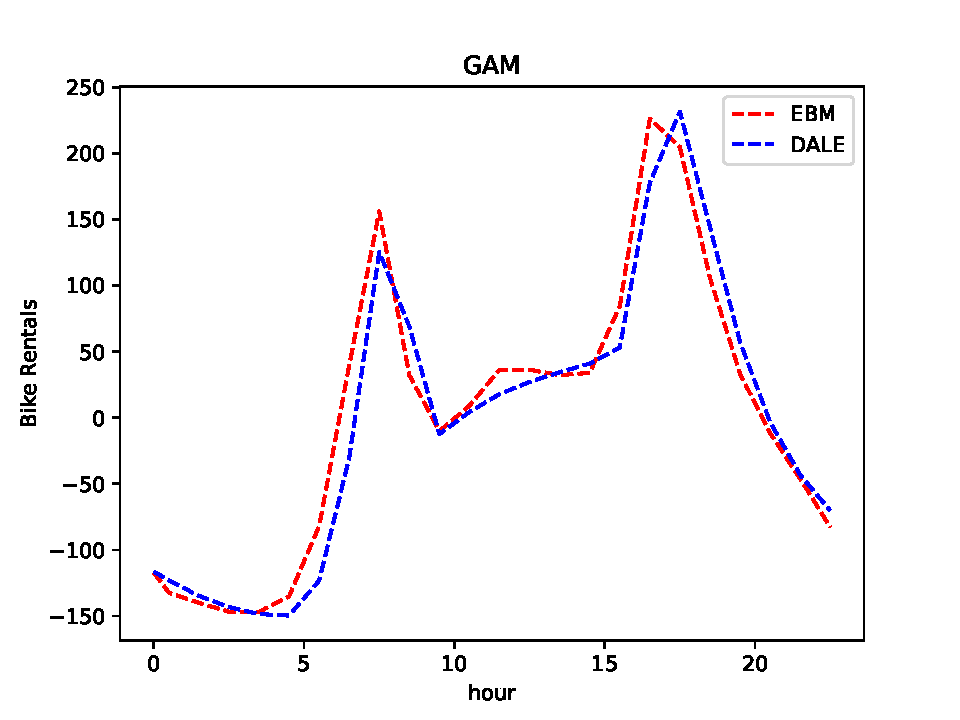
\includegraphics[width=\textwidth]{figures/bike_rentals_gam}
        \caption{\(f(X_{\mathtt{hour}})\)}
        \label{subfig:bike_rentals_gam}
    \end{subfigure}
    \begin{subfigure}{0.32\textwidth}
        \centering
        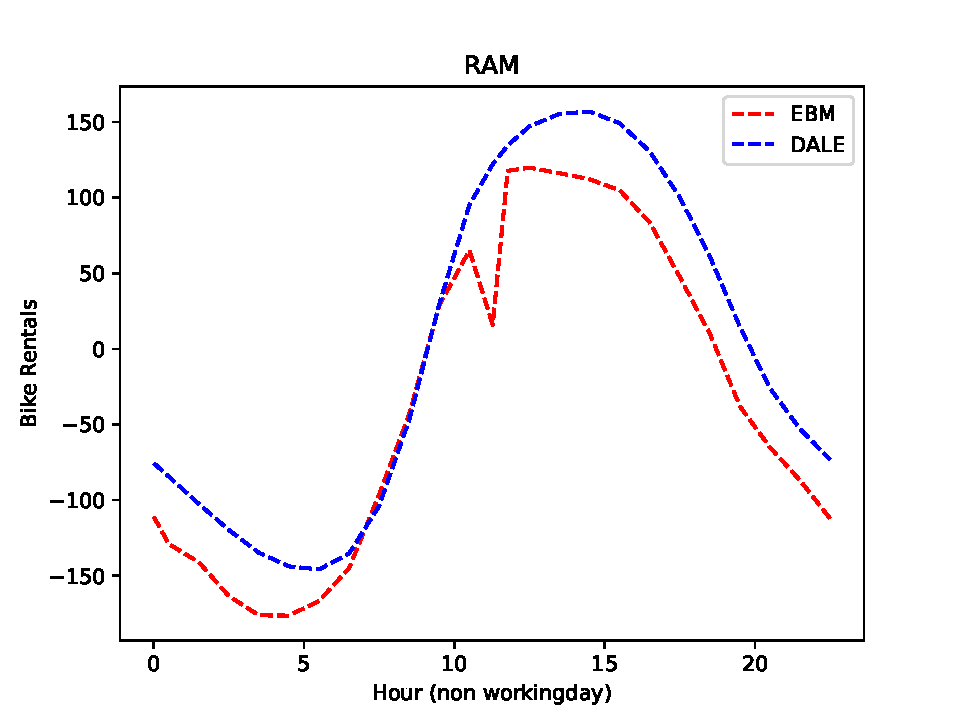
\includegraphics[width=\textwidth]{figures/bike_rentals_ram_1}
        \caption{\(f(X_{\mathtt{hour}}) \when{X_{\mathtt{workingday}} \neq 1}\)}
        \label{subfig:bike_rentals_regional_gam_1}
    \end{subfigure}
    \begin{subfigure}{0.32\textwidth}
        \centering
        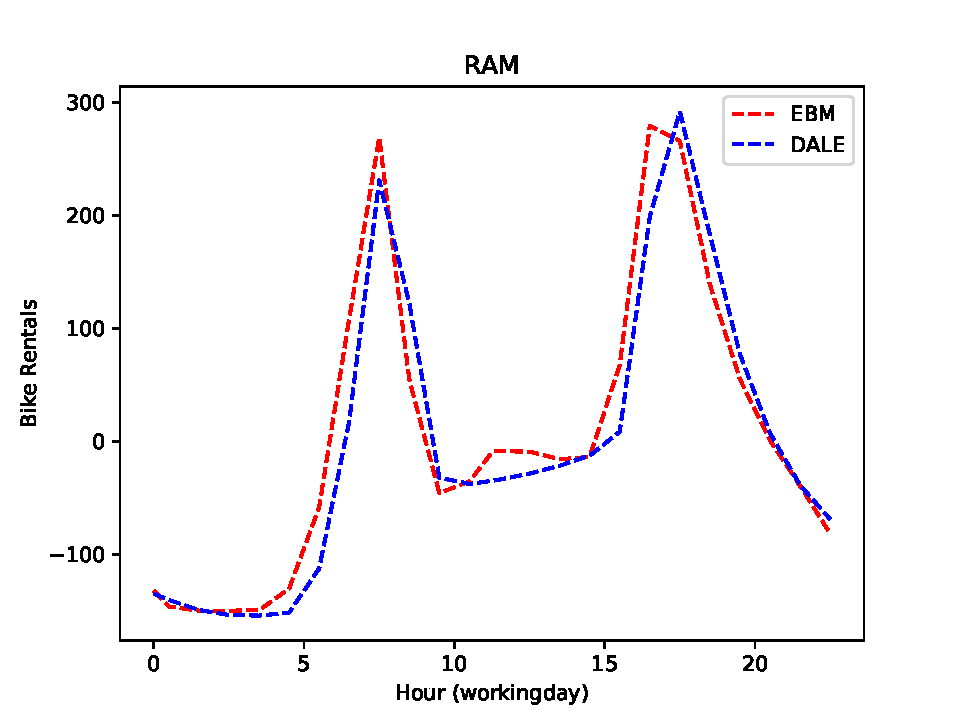
\includegraphics[width=\textwidth]{figures/bike_rentals_ram_2}
        \caption{\(f(X_{\mathtt{hour}}) \when{X_{\mathtt{workingday}} = 1}\)}
        \label{subfig:bike_rentals_regional_gam_2}
    \end{subfigure}
    \label{fig:bike_sharing}
\end{figure}

\end{frame}


\begin{frame}
  \frametitle{Experimental Results}

  Tested on \href{https://archive.ics.uci.edu/dataset/275/bike+sharing+dataset}{Bike Sharing} and \href{https://inria.github.io/scikit-learn-mooc/python_scripts/datasets_california_housing.html}{California Housing} Datasets.

\noindent\makebox[\linewidth]{\rule{\paperwidth}{0.4pt}}

\begin{table}[htbp]
  \centering
  \label{tab:sample}
  \begin{tabular}{l|c|cccc}
      & \textbf{Black-box} & \multicolumn{4}{c}{\textbf{x-by-design}} \\
      \hline
      \hline
      & all orders & \multicolumn{2}{c}{1\textsuperscript{st} order} & \multicolumn{2}{c}{2\textsuperscript{nd} order} \\
      \hline
      \hline
      & \textbf{DNN} & \textbf{GAM} & \textbf{RAM} & \textbf{GA}$^2$\textbf{M} & \textbf{RA}$^2$\textbf{M} \\
      \hline
      Bike (MAE)  & 0.254 & 0.549 & \textbf{0.430} & 0.298 & \textbf{0.278} \\
      Bike (RMSE) & 0.389 & 0.734 & \textbf{0.563} & 0.438 & \textbf{0.412} \\
      \hline
      Housing (MAE)  & 0.373 & 0.600 & \textbf{0.553} & 0.554 & \textbf{0.533} \\
      Housing (RMSE) & 0.533 & 0.819 & \textbf{0.754} & 0.774 & \textbf{0.739} \\
  \end{tabular}
\end{table}

\end{frame}


\begin{frame}
  \frametitle{What is next?}
  \begin{itemize}
  \item Results are preliminary
    \begin{itemize}
      \item Compare $RAM$ vs $GAM$ and $RA^2M$ vs $GA^2M$ in more datasets
      \item Check robustness on edge cases:
        \begin{itemize}
        \item highly correlated features
        \item limited training examples
        \end{itemize}
      \end{itemize}

    \item Can we model uncertainty?
      \begin{itemize}
      \item Uncertain because we do not model higher-order interactions
      \item Uncertain about the conditionals, i.e., detected subregions
      \item Uncertain about the univariate functions we learn
      \end{itemize}

    \item Could we make it a 1-step process?
      \begin{itemize}
        \item a network that automatically learns both the univariate functions and the conditions
      \end{itemize}
  \end{itemize}

  \noindent\makebox[\linewidth]{\rule{\paperwidth}{0.4pt}}

\end{frame}


\begin{frame}
  \frametitle{Thank you for your attention}
  \begin{itemize}
  \item For more discussion or future ideas on RAM, contact me:
    \begin{itemize}
    \item \href{vgkolemis@athenarc.gr}{vgkolemis@athenarc.gr}
    \item \href{gkolemis@hua.gr}{gkolemis@hua.gr}
    \end{itemize}
  \item More info about the paper:
\begin{figure}[htbp]
  \centering
  
\includegraphics[width=.2\textwidth]{figures/publications}
\end{figure}
  \item Questions?
  \end{itemize}


\end{frame}



% \begin{frame}[allowframebreaks]
%   \frametitle{References}
%   \printbibliography
% \end{frame}


\end{document}